\documentclass[11pt,a4paper]{article}

\usepackage[utf8]{inputenc}
\usepackage[T1]{fontenc}
\usepackage[margin=2.2cm]{geometry}
\usepackage{parskip}
\usepackage{titlesec}
\usepackage{enumitem}
\usepackage{booktabs}
\usepackage{xcolor}
\usepackage{tcolorbox}
\usepackage{graphicx}
\usepackage{hyperref}
\usepackage{fancyhdr}
\usepackage{listings}
\usepackage{longtable}
\usepackage{array}

\tcbuselibrary{skins,breakable}

\definecolor{accent}{RGB}{30,80,150}
\definecolor{softgray}{RGB}{245,246,248}
\definecolor{codebg}{RGB}{248,248,250}
\definecolor{warn}{RGB}{160,60,40}
\definecolor{good}{RGB}{30,120,70}

\titleformat{\section}{\Large\bfseries\color{accent}}{\thesection}{0.8em}{}
\titleformat{\subsection}{\large\bfseries}{\thesubsection}{0.6em}{}
\titleformat{\subsubsection}{\normalsize\bfseries\itshape}{\thesubsubsection}{0.5em}{}

\hypersetup{
  colorlinks=true, linkcolor=accent, urlcolor=accent,
  pdftitle={AgentIA --- System Review, Verification and Cost Report},
  pdfauthor={AgentIA Engineering}
}

\pagestyle{fancy}
\fancyhf{}
\fancyhead[L]{\small\color{accent}AgentIA --- System Review}
\fancyhead[R]{\small\color{accent}\thepage}
\renewcommand{\headrulewidth}{0.4pt}

\lstset{
  basicstyle=\ttfamily\small, backgroundcolor=\color{codebg},
  frame=single, rulecolor=\color{softgray}, breaklines=true,
  columns=fullflexible, keepspaces=true, showstringspaces=false,
  xleftmargin=0.5em, xrightmargin=0.5em,
}

\newtcolorbox{notebox}[1][]{colback=softgray,colframe=accent,boxrule=0.4pt,
  arc=2pt,left=6pt,right=6pt,top=4pt,bottom=4pt,breakable,#1}

\title{\vspace{-1.4cm}\textbf{AgentIA --- System Review, Verification and Cost}\\[0.25cm]
\large The agentic workflow, the orchestration, what is measured, and what it costs}
\author{AgentIA Engineering}
\date{2026-09-29}

\begin{document}
\maketitle
\thispagestyle{fancy}

\begin{notebox}
\textbf{What this document is.} A review of the system as it actually runs today:
the agentic generation workflow (the LangGraph pipeline and its verification loop),
the orchestration around it, the design, the verification results obtained this
week, and a cost/usage report gathered from the platform's own stores --- the local
SQLite system of record and its MLflow mirror.

It is written \emph{after} the platform produced its first verified builds, so it
separates what is measured from what is asserted. Where the two cost sources
disagree, this document says so rather than picking one silently.
\end{notebox}

\tableofcontents
\vspace{0.4cm}

\section{Executive summary}

Four facts dominate this review.

\begin{enumerate}[leftmargin=1.4em]
  \item \textbf{The platform now verifies its own output.} Until this week the
  system reported ``0 of 15 sessions verified''. The cause was a one-character
  Docker mount defect (a private SELinux relabel concatenated onto a read-only
  flag, producing an invalid mount option that made every build exit before Maven
  ran). It is fixed, and the first verified builds are on record.
  \item \textbf{The agentic workflow is real and governed.} A LangGraph state
  machine runs eight nodes --- validator, five generation stages, sandbox, repair
  --- with a deterministic compliance gate at every stage and a bounded repair
  loop. Every generation stage has two implementations, \texttt{MODEL} and
  \texttt{DETERMINISTIC}, dispatched once per session.
  \item \textbf{Verification-guided selection is the measured reliability lever.}
  With a single sample the generator builds 78\% of the time; sampling three
  candidates and keeping the first that builds raises task-level coverage to 100\%
  at \$0.20 per reliable service.
  \item \textbf{The verifier is intermittently flaky, and the cost mirror has
  drifted.} The same frozen workspace rebuilds 4-of-6 times under load and 8-of-8
  times sequentially; the leading cause is the same mount configuration. And the
  MLflow mirror undercounts the system of record by $\approx$\$1.6 (20\%), so the local
  store --- not the mirror --- is the number to quote.
\end{enumerate}

\section{The agentic workflow}

\subsection{The pipeline as a state machine}

Generation is a LangGraph state machine of eight nodes (\texttt{graph.py}). The
topology is a linear spine with exactly one bounded cycle, shown in
Figure~\ref{fig:workflow}:

\begin{center}
\texttt{validator $\rightarrow$ scaffolder $\rightarrow$ domain $\rightarrow$ service
$\rightarrow$ controller $\rightarrow$ test $\rightarrow$ sandbox
$\rightleftharpoons$ repair}
\end{center}

Each generation node emits one file (or a small set of files) into a shared
workspace; the sandbox then compiles and tests the whole project hermetically; on
failure the repair node applies a surgical patch and the sandbox runs again, bounded
by a maximum attempt count.

\subsection{Dual implementation: MODEL and DETERMINISTIC}

Every generation stage has two implementations (\texttt{stages/deterministic/} and
\texttt{stages/model/}), selected once per session by
\texttt{select\_generation\_mode()}. The decision is recorded in the state and never
re-decided mid-session, so a session cannot produce a hybrid of template-shaped and
model-shaped artifacts. The deterministic path emits offline templates with zero
model calls and is byte-identical across runs; the model path drives a commodity LLM
(currently \texttt{deepseek-flash}) with a versioned instruction set.

\subsection{The compliance gate}

Before any stage's candidate is persisted it passes a merged compliance gate
(\texttt{stages/compliance.py}): the test-analysis validator family and the security
architecture validator family are combined, and every finding carries an attribution
--- \texttt{LOCAL} (this stage owns the offending artifact) or \texttt{ACCUMULATED}
(no single stage owns it). Blocking local violations reject the candidate and consume
a correction attempt; accumulated findings are recorded but never reject. This split
is what keeps a whole-project concern from being blamed on one stage.

\subsection{The verification sandbox}

The sandbox (\texttt{workspace\_verification.py}) runs, in order: strip
version-control metadata; inject a platform-authored persistence contract test (a
\texttt{@SpringBootTest} with \texttt{ddl-auto=validate} against the generated
\texttt{schema.sql}); then \texttt{docker run --rm --network none ... mvn test -o}
against a read-only Maven cache. The contract test is the acceptance signal the
generator cannot author: the model never sees it, and a schema/entity contradiction
fails the build even though every model-written unit test (which mocks the
repository) passes. Test counts are parsed from the build's own surefire summary
rather than fabricated.

\subsection{Bounded self-repair}

On build failure the repair node parses the Maven trace
(\texttt{repair.py}, \texttt{repair\_parser.py}) into a failure class
(compilation, assertion, runtime) and applies a surgical unified patch, then re-enters
the sandbox. The attempt cap is 3 in the constitution and 5 in
\texttt{config.py:73} --- a live inconsistency noted in Section~\ref{sec:findings}.

\section{Orchestration}

\subsection{Two entry points, one product}

The system exposes two ways to start a session, and this review confirms both now
reach the model and both verify the workspace:

\begin{itemize}[leftmargin=1.4em]
  \item \textbf{Graph path} --- \texttt{POST /sessions} enqueues a session whose
  worker runs the compiled graph end to end, credentials threaded through the
  \texttt{X-LLM-API-Key} header.
  \item \textbf{Sequential path} --- \texttt{POST /sessions/quick-start} with
  \texttt{autoRun}, and \texttt{/orchestrator/pipeline/run}, drive
  \texttt{pipeline\_runner}, which runs the same generation stages, the same
  hermetic verification, a static security audit, and DevOps/export phases.
\end{itemize}

The sequential path previously generated code and \emph{never compiled it}; it now
runs the same verification seam as the graph, so the two paths cannot drift.

\subsection{Queue, lifecycle and streaming}

A FIFO queue (\texttt{queue\_service.py}) caps concurrency at two simultaneous
sandbox executions. The lifecycle (\texttt{lifecycle\_service.py}) walks
\texttt{REQUIREMENTS $\rightarrow$ ARCHITECTURE $\rightarrow$ DATA\_MODEL
$\rightarrow$ CODE\_TESTS $\rightarrow$ SECURITY\_AUDIT $\rightarrow$ DEVOPS
$\rightarrow$ EXPORT $\rightarrow$ COMPLETED}, with in-flight pause, resume and cancel
and live Server-Sent-Events streaming to the monitor screen.

\subsection{Measurement and self-improvement substrate}

Two further layers sit alongside generation. The diagnostic instrument
(\texttt{conformance\_diagnostics.py}) is a deterministic, rule-attributed scorer
that persists one durable record per session and produces a corpus report. The
skill-optimisation loop (features 014--015) is \emph{built} --- collect, reflect,
apply, a strict-improvement gate, per-skill contribution by leave-one-out, and
eviction with an evidence floor --- but it is deliberately not run, for the reasons
stated in Section~\ref{sec:verification}.

\section{Design}

\begin{figure}[htbp]
  \centering
  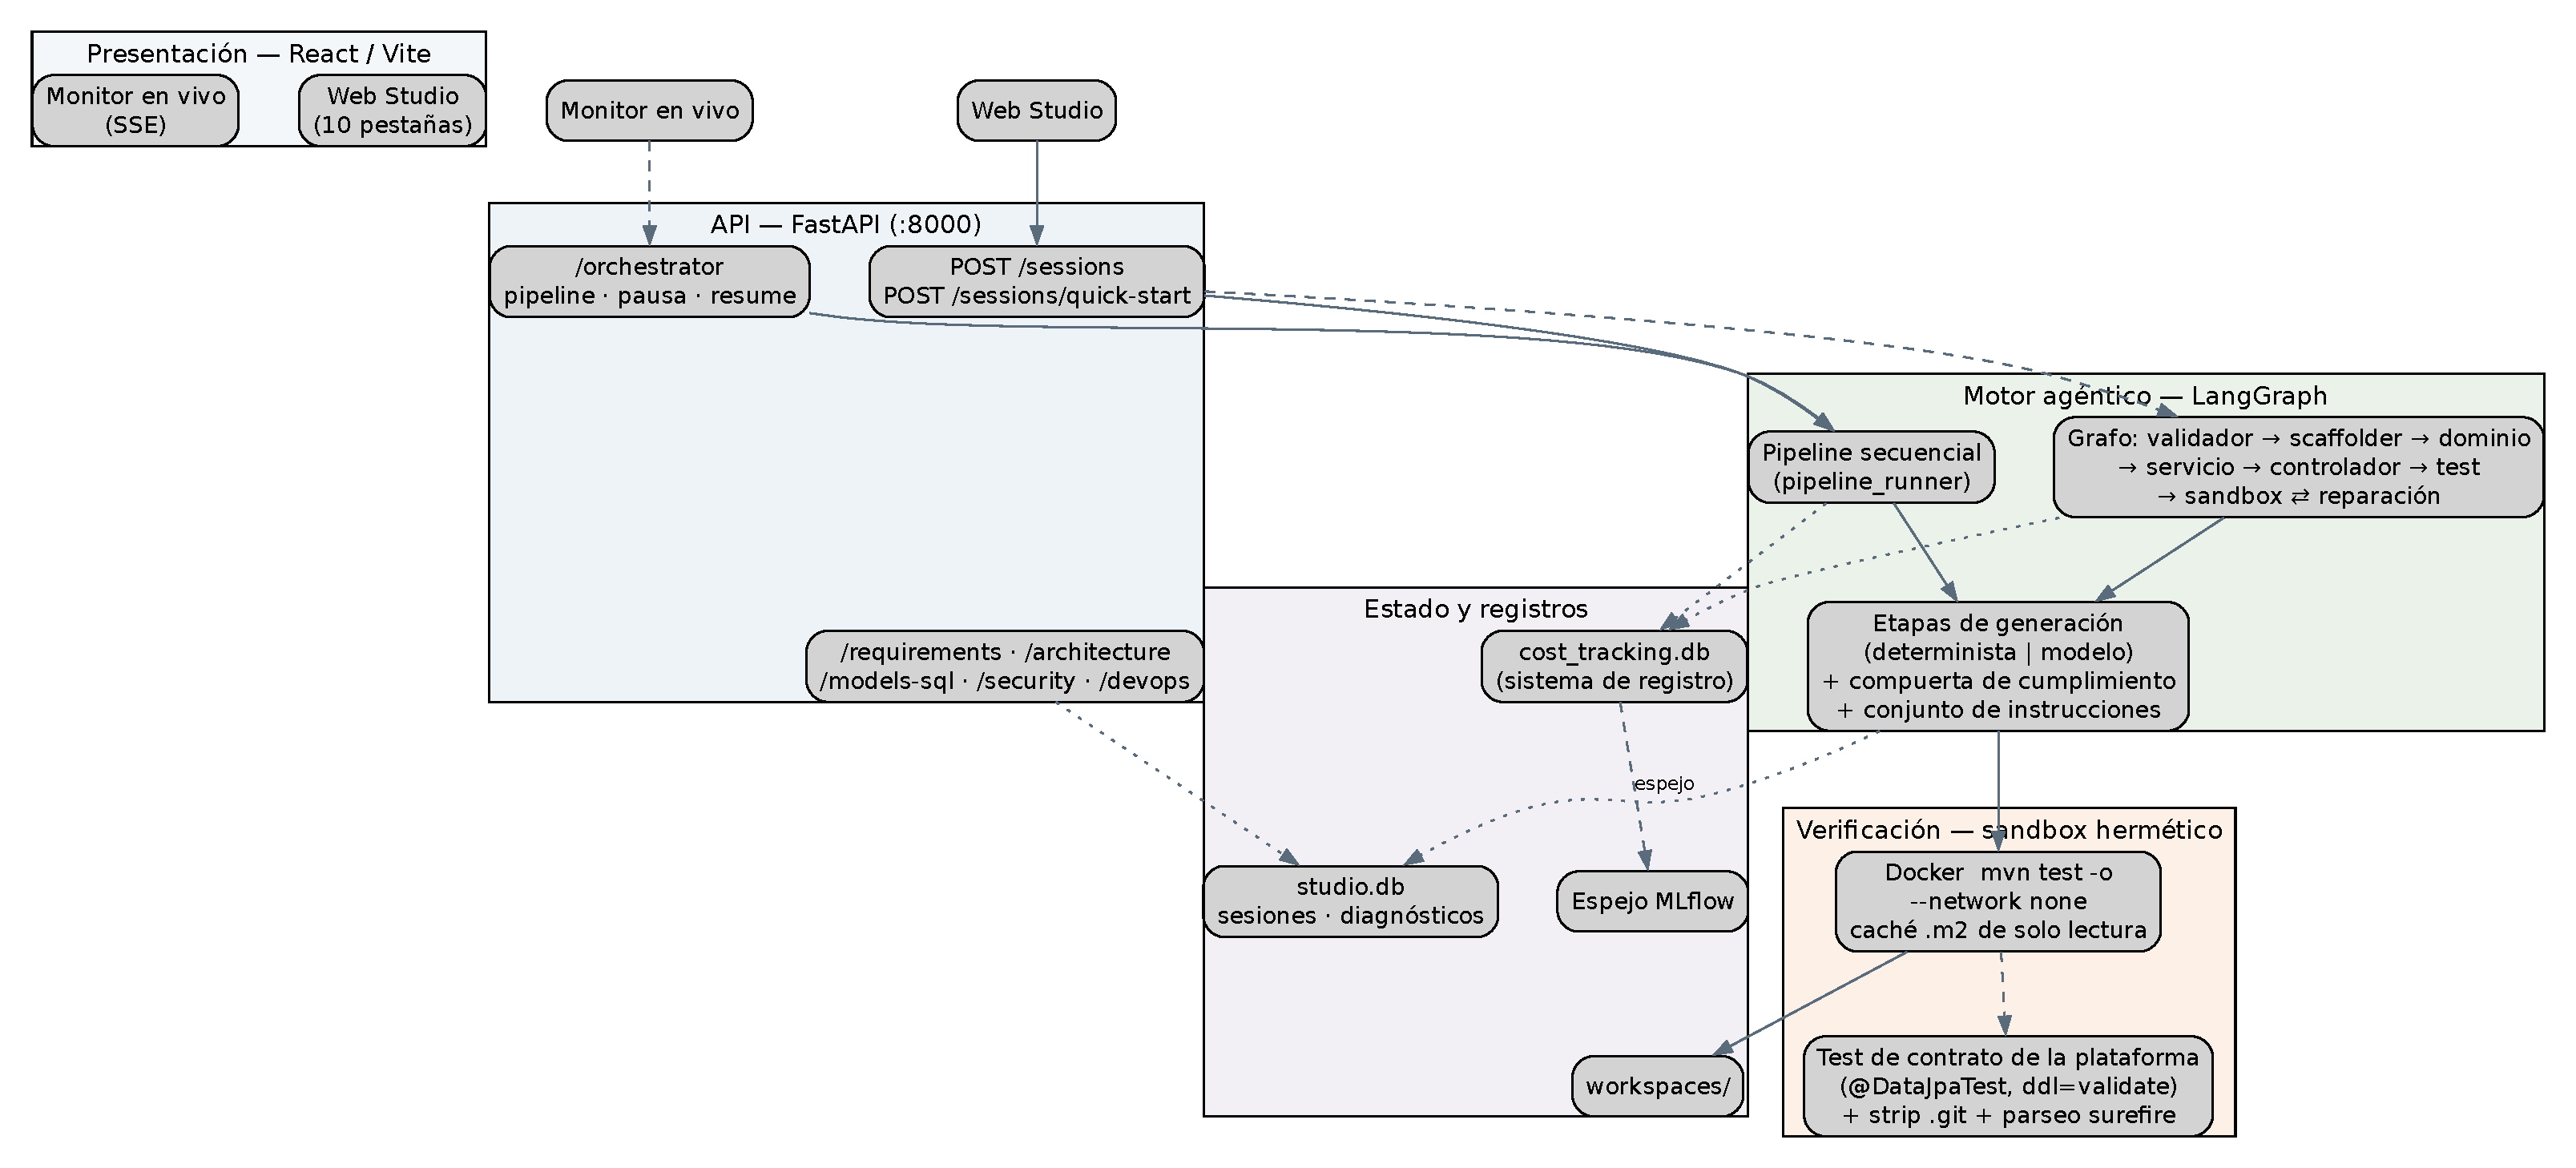
\includegraphics[width=\linewidth]{fig/architecture.pdf}
  \caption{System architecture: the React studio over the FastAPI API, the LangGraph
  agentic engine, the hermetic verification sandbox, and the state/cost stores.}
  \label{fig:architecture}
\end{figure}

\begin{figure}[htbp]
  \centering
  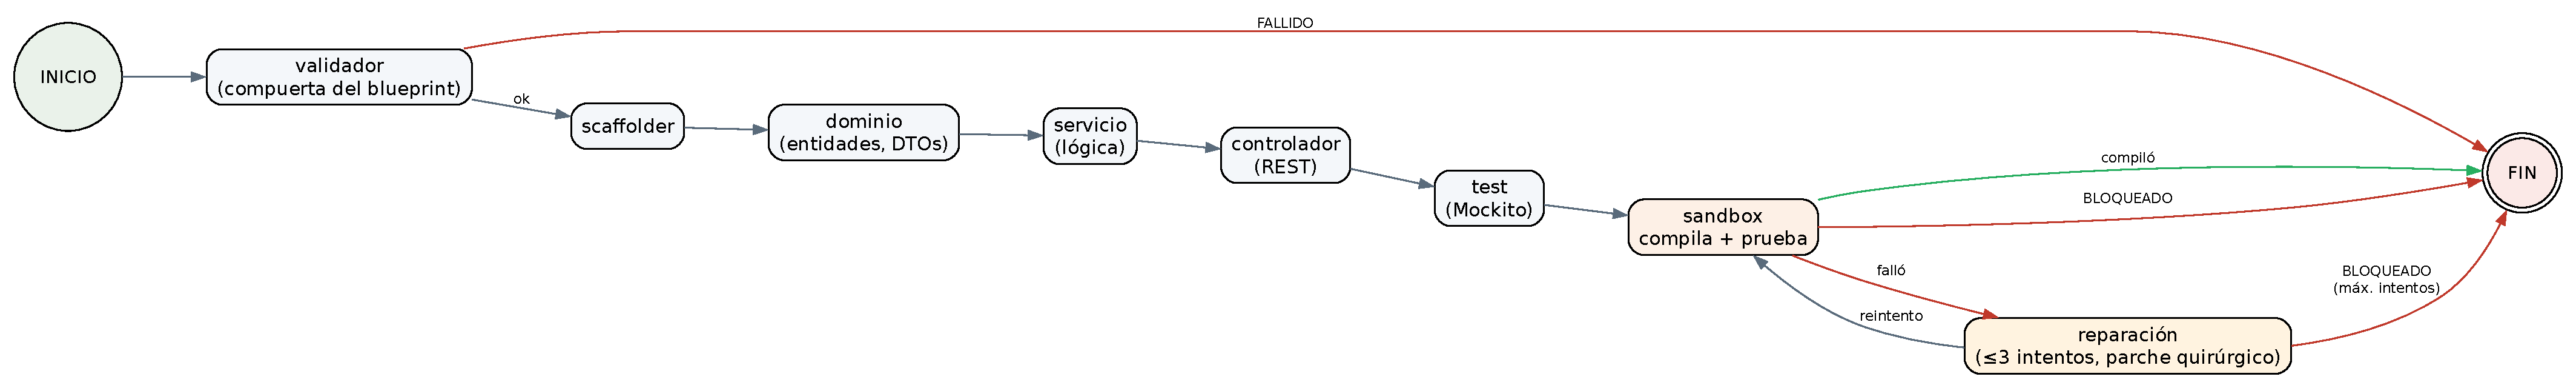
\includegraphics[width=0.82\linewidth]{fig/workflow.pdf}
  \caption{The generation state machine: a linear spine with one bounded
  repair--sandbox cycle.}
  \label{fig:workflow}
\end{figure}

\subsection{Service inventory}

\begin{center}
\begin{longtable}{@{}p{0.34\textwidth}p{0.60\textwidth}@{}}
\toprule
\textbf{Service} & \textbf{Role} \\
\midrule
\texttt{requirements\_service} & BDD story decomposition and spec synthesis \\
\texttt{architecture\_service} & 4-layer architecture and component catalogue \\
\texttt{model\_sql\_service} & JPA entities, DTOs, schema/data SQL, ER diagram \\
\texttt{test\_analysis\_service} & static constitutional-rule analyser (family A) \\
\texttt{security\_service} & SAST, secrets, architecture conformance (family B) \\
\texttt{conformance\_diagnostics} & deterministic rule-attributed conformance scorer \\
\texttt{corpus\_report} & batch/corpus measurement report \\
\texttt{workspace\_verification} & strip VCS, inject contract test, run the build \\
\texttt{verification\_selection} & best-of-$k$: generate, verify, stop at first pass \\
\texttt{platform\_verification} & platform-authored persistence contract test \\
\texttt{skill\_contribution} & leave-one-out per-skill contribution \\
\texttt{llm\_factory} & provider detection and model-client construction \\
\texttt{structured\_output} & schema-constrained model output \\
\texttt{injection\_guard} & prompt-injection defence for the reflector \\
\texttt{queue\_service / lifecycle\_service} & concurrency and phase orchestration \\
\texttt{docker\_service / devops / export / git} & container deploy, CI, ZIP, publish \\
\texttt{cost recording + mlflow sink} & per-call and per-session cost, mirror \\
\bottomrule
\end{longtable}
\end{center}

\section{Verification results}
\label{sec:verification}

\subsection{Coverage scaling: the reliability lever}

Verification-guided selection --- generate $k$ candidates, verify each, keep the
first that passes --- is measured here, not borrowed from another task class. The
control arm of this week's experiment is 6 tasks, each resampled 3--4 times with the
same instructions and model; the coverage formula is
$\mathrm{coverage}(k)=1-(1-p)^k$ (\emph{Large Language Monkeys},
\texttt{arXiv:2407.21787}).

\begin{center}
\begin{tabular}{@{}lrl@{}}
\toprule
\textbf{Metric} & \textbf{Value} & \\
\midrule
pass@1 (single sample) & \textbf{78.3\%} & \\
coverage $k{=}1$ & 83.3\% & \\
coverage $k{=}2$ & 83.3\% & \\
coverage $k{=}3$ & \textbf{100.0\%} & 6 of 6 tasks \\
coverage $k{=}4$ & 100.0\% & \\
\bottomrule
\end{tabular}
\end{center}

At \$0.065 per generated service, three candidates cost \textbf{\$0.20 per reliable
service}. Caveats, stated not smoothed: $n{=}6$ tasks, one model, one provider; this
is a demonstration of the lever, not a benchmark, and the direction (coverage is
monotone in $k$) is robust while the 100\% is ``6 of 6 tasks''.

\subsection{The verifier is intermittently flaky}

The same frozen workspace, rebuilt under load earlier, passed 4 of 6 times; rebuilt
sequentially, two workspaces passed 8 of 8 each. The failure, when it occurs, is a
surefire \texttt{PluginContainerException} on a \texttt{surefire-shared-utils}
foreign import --- \emph{after} every test has passed.

The flake is therefore not a per-workspace code defect. It is intermittent and
load-correlated, and the leading hypothesis is the mount configuration:
\texttt{DOCKER\_MOUNT\_SUFFIX=:Z} is a \emph{private} SELinux relabel, correct for a
per-session workspace but wrong for a \emph{shared read-only Maven cache} mounted by
many concurrent containers. Two containers relabelling one shared source with
\texttt{:Z} is a known cause of exactly this class of intermittent class-realm
failure. The proposed fix is to apply \texttt{:Z} to the workspace only and leave the
cache unrelabelled (or \texttt{:z}), confirmed by a repeatability gate.

\begin{notebox}[colframe=warn]
\textbf{Why this gates everything downstream.} A verifier that flips $\approx$ 33\% of
runs cannot serve as an admission oracle: coverage would over-promise, an admission
gate would promote noise, and Ratchet's theorem (\texttt{arXiv:2605.22148}) says a
judge this noisy retires nothing at any sample size. Making the oracle deterministic
is therefore the prerequisite for every further measurement --- including the
skill-optimisation loop, which stays closed behind it.
\end{notebox}

\section{Cost and usage}
\label{sec:cost}

Costs are recorded per call and per session in the local SQLite store
(\texttt{backend/cost\_tracking.db}), which is the \textbf{system of record}, and
mirrored into MLflow (\texttt{mlflow.db}). The two are compared here, not merged.

\subsection{System of record (authoritative)}

\begin{center}
\begin{tabular}{@{}lrrr@{}}
\toprule
\textbf{Scope} & \textbf{Calls} & \textbf{Cost (USD)} & \textbf{Output tokens} \\
\midrule
Polarity experiment (\texttt{p4}) & 750 & \textbf{6.58} & --- \\
Frozen-five baseline (\texttt{corpus}) & 120 & 0.63 & --- \\
Hard ten & 50 & 0.64 & --- \\
Probes / single sessions & $\approx$ 250 & $\approx$ 0.16 & --- \\
\midrule
\textbf{Total} & \textbf{1172} & \textbf{8.01} & \textbf{12.28M} \\
\bottomrule
\end{tabular}
\end{center}

All 1172 calls were \texttt{deepseek-flash}. Total input tokens 6.45M, output tokens
12.28M. The single dominant cost is the instruction-polarity experiment, which is a
finished measurement (a null), not an ongoing drain.

\subsection{MLflow mirror (and where it has drifted)}

\begin{center}
\begin{tabular}{@{}lrrrr@{}}
\toprule
\textbf{Experiment} & \textbf{Runs} & \textbf{Cost (USD)} & \textbf{In tok} & \textbf{Out tok} \\
\midrule
\texttt{Default} (legacy) & 877 & 5.41 & 4.63M & 8.20M \\
\texttt{agentia} (current) & 114 & 0.98 & 0.78M & 1.52M \\
\midrule
\textbf{Mirror total} & 991 & \textbf{6.39} & 5.40M & 9.72M \\
\bottomrule
\end{tabular}
\end{center}

\begin{notebox}[colframe=warn]
\textbf{The mirror has drifted.} MLflow totals \textbf{\$6.39} against the system of
record's \textbf{\$8.01} --- an undercount of $\approx$\$1.62 (20\%), with $\approx$ 181 fewer
calls and token totals that also disagree. The mirror is split across a legacy and a
current experiment, and only per-call metrics are being written (session aggregates
are absent). The earlier ``the mirror works and it agrees'' claim is no longer true
for the current data. Until the sink is repaired, the local store is the only number
to quote, and a cost report generated from MLflow alone would understate spend.
\end{notebox}

\section{Findings and next steps}
\label{sec:findings}

\begin{enumerate}[leftmargin=1.4em]
  \item \textbf{Make the verifier deterministic before spending anything more.}
  Split the mount suffix (workspace \texttt{:Z}, shared cache unrelabelled) and add a
  repeatability gate: one frozen workspace must rebuild $N/N$ times.
  \item \textbf{Make the measure able to move.} The conformance instrument reads 0 on
  failing builds; surface the repair parser's failure classes as accumulated
  findings so a build failure is attributable.
  \item \textbf{Use verification-guided selection as the reliability mechanism now.}
  It is measured (\$0.20/service at $k{=}3$), it needs no training, and it is the
  lever the literature ranks first.
  \item \textbf{Repair the cost mirror.} Session-level mirroring is not populating;
  restore it or the MLflow UI understates spend.
  \item \textbf{Resolve the repair-cap inconsistency} (constitution 3 vs
  \texttt{config.py} 5).
  \item \textbf{Leave the skill-optimisation loop closed} until items 1 and 2 pass
  their gates; the instruction-polarity experiment that was its most promising
  input is a null (prohibition vs control: 1 win, 3 losses, 2 ties).
\end{enumerate}

\end{document}
